\chapter{The SEXTANTE history manager}

\section {Introduction}

Every time you execute a SEXTANTE algorithm, information about the process is stored in the SEXTANTE history manager. Along with the parameters used, the date and time of the execution are also saved.

This way, it is easy to track the and control all the work that has been developed using SEXTANTE, and easily reproduce it.

The SEXTANTE history manager is a set of registry entries grouped according to their date of execution, making it easier to find information about an algorithm executed at any particular moment.

\begin{center}
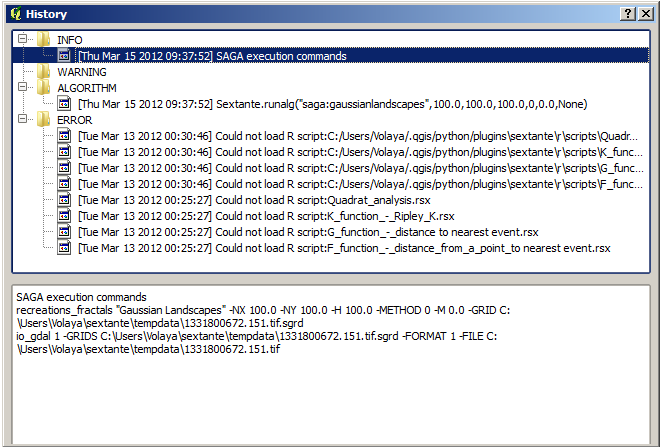
\includegraphics[width=.4\columnwidth]{history.png}
\end{center}

Process information is kept as a command--line expression, even if the algorithm was launched from the toolbox. This makes it also useful for those learning how to use the command--lin interface, since they can call an algorithm using the toolbox and then check the history manager to see how that same algorithm could be called from the command line.

Apart from browsing the entries in the registry, processes can be re--executed, simply double--clicking on the corresponding entry.

Along with algorithm executions, SEXTANTE communicates with the user using the other groups of the registry, namely \emph{Errors, Warnings} and \empg{Information}. In case something is not working properly, having a look at the \emph{Errors} might help you to see what is happening. If you get in contact with a SEXTANTE developer to report a bug or error, the information in that group will be very useful for him to find out what is going wrong.

Some algorithms, even if they can produce a result with the given input data, might add comments or additional information to \emph{Warning} in case they detect potential problems from that data, in order to warn you about them. Make sure you check those messages in case you are having unexpected results.